%%%%%%%%%%%%%%%%%%%%%%%%%%%%%%%%%%%%%%%%%%%%%%%%%%%
%% LaTeX book template 
%%%%%%%%%%%%%%%%%%%%%%%%%%%%%%%%%%%%%%%%%%%%%%%%%%%

\documentclass[a4paper,11pt]{book}
\usepackage[T1]{fontenc}
\usepackage[utf8]{inputenc}
\usepackage{lmodern}
\usepackage{hyperref}
\usepackage{graphicx}
\usepackage[english]{babel}
\usepackage{amsmath}
\usepackage{amssymb}
\usepackage{amsthm}
\newtheorem{theorem}{Theorem}
\newtheorem{definition}{Definition}

\newenvironment{dedication}
{
   \cleardoublepage
   \thispagestyle{empty}
   \vspace*{\stretch{1}}
   \hfill\begin{minipage}[t]{0.66\textwidth}
   \raggedright
}
{
   \end{minipage}
   \vspace*{\stretch{3}}
   \clearpage
}

\makeatletter
\renewcommand{\@chapapp}{}% Not necessary...
\newenvironment{chapquote}[2][2em]
  {\setlength{\@tempdima}{#1}%
   \def\chapquote@author{#2}%
   \parshape 1 \@tempdima \dimexpr\textwidth-2\@tempdima\relax%
   \itshape}
  {\par\normalfont\hfill--\ \chapquote@author\hspace*{\@tempdima}\par\bigskip}
\makeatother

\title{\Huge \textbf{Neural dynamics of vision}  \\ \huge A computational perspective}

\author{\textsc{Clayton Seitz}\thanks{\url{cwseitz.github.io}}}

\begin{document}

\frontmatter
\maketitle

\begin{dedication}
Dedicated to Calvin and Hobbes.
\end{dedication}

\tableofcontents
\mainmatter

\chapter{The Neural Code}

\section{Introduction}

Throughout this section of the text we will coarsely examine the biophysical properties of the elements of the nervous systems: neurons. The hope is that by introducing the nervous system from a physical perspective, much of the mathematical developments in later chapters will seem natural and well-motivated. However, we will see that much of the later work neglects many of the features of neurons this chapter will introduce and for good reason. It never hurts to know what you have left out of your model.

Neurons are one of the most interesting cell types in animals particularly for their evolved ability to sense their external environment and produce a myriad of responses in favor of the survival of the host organism. All vertebrates have a distinct central nervous system consisting of a brain and a spinal cord which process information from or send information to a peripheral nervous system. Here we will discuss the cellular elements that allow neurons to send information to each other in such a system.

\section{Neuroelectronics}

Neurons are bounded by a 3-4nm thick membrane composed of a diverse set of lipids forming a bi-layer and are submerged in a bath of water and ions $\it{in \;vivo}$. These cells have evolved a vast array of membrane ion channels that control the concentrations of ions on either side of the membrane. The degree to which these channels allow ions to flow in and out of the membrane is the basis of all neural processing and in turn all of our actions and conscious awareness. 

\subsection{RC Model}

A well-known model of a neuron membrane is an RC circuit where the resistor represents a sort of permeability of the membrane to ions while the capacitor models the membrane itself. Since either side of the membrane contains electrically charged ions there exists an electrical potential in these regions and in turn a potential difference across the lipid bi-layer. The current through the membrane is ultimately determined by the balance between diffusion of ions down their concentration gradients and electrical potential gradients. 

\begin{figure}
\centering
  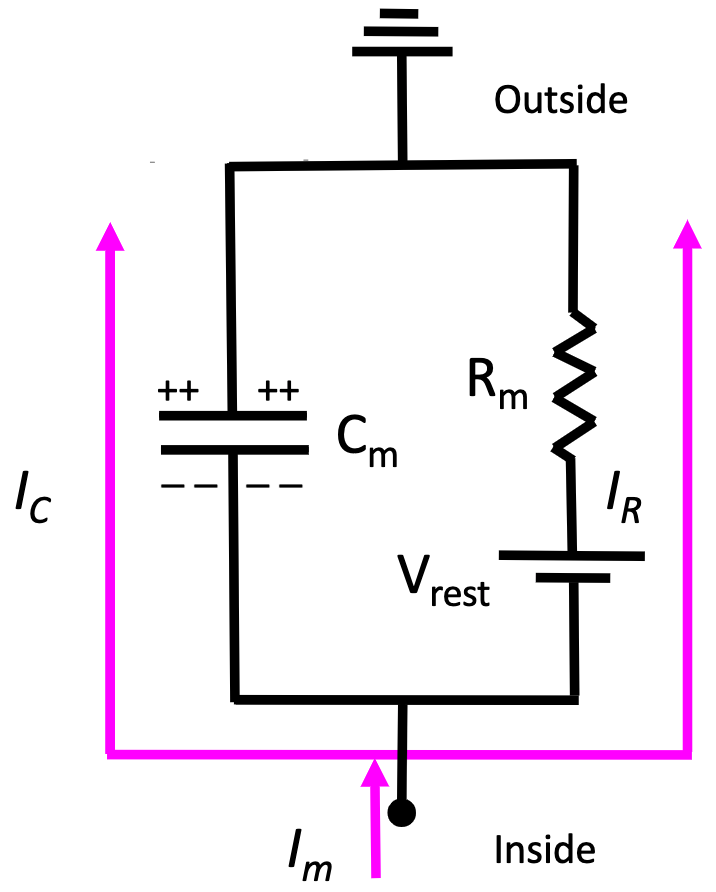
\includegraphics[width=3in]{assets/circuit-model.png}
  \caption{RC Circuit Model}
  \label{fig:circuit}
\end{figure}

If we inject a current $I_{E}$ into the cell, by conservation of current we have

\begin{eqnarray*}
I_{E} &=& C\frac{dV}{dt} + I_{R}\\
\end{eqnarray*}

where $V$ is the membrane voltage. We can also use Maxwell's equations (Kirchhoff's voltage rule) to write

\begin{eqnarray*}
I_{R} &=& \frac{V-V_{0}}{R}\\
\end{eqnarray*}


where have replaced the resistance by the conductance $g$. Combining these two equations we are left with the following differential equation for the membrane voltage.

\begin{eqnarray*}
C\frac{dV}{dt} &=& I_{E} - \frac{V - V_{0}}{R}\\
\end{eqnarray*}

which is commonly rewritten by defining the membrane time constant $\tau = RC$

\begin{eqnarray*}
\tau\frac{dV_{C}}{dt} &=& I_{E}R - (V - V_{0})\\
\end{eqnarray*}

Notice that as $t\rightarrow \infty$ we have $V_{C}-V_{rest} \rightarrow I_{E}R + V_{0}$ and so we define the steady-state voltage $V_{\infty} = I_{E}R + V_{0}$. Inserting this new definition into the equation

\begin{eqnarray*}
\tau\frac{dV}{dt} &=& V_{\infty} - V\\
\end{eqnarray*}

which can be solved to give

\begin{eqnarray*}
V(t) &=& V_{\infty}(1-e^{-\frac{t}{\tau}})\\
\end{eqnarray*}

\subsection{Equilibrium and Reversal Potentials}

The flux of ions through the cell membrane is due to an imbalance of electrical and chemical potentials. Recall the Boltzmann distribution of energies at a temperature $T$

\begin{equation*}
P(\epsilon) = \frac{e^{-\frac{\epsilon}{k_{B}T}}}{Z}
\end{equation*}

where the partition function $Z= \int e^{-\frac{\epsilon}{k_{B}T}}d\epsilon$. We define the $\mathbf{reversal\; potential}$ as the membrane potential at which electrical forces perfectly balance the diffusion of ions down their concentration gradient and their is no current through the membrane. We compute this using the famous Nernst equation

\begin{equation*}
E = \frac{RT}{zF}\ln \frac{[o]}{[i]}
\end{equation*}

Perhaps we would rather compute the resting potential of the membrane with knowledge of the concentrations of ions inside and outside of the cell. For a set of positive ions $M$ and negative ions $A$

\begin{equation*}
E = \frac{RT}{F}\ln \frac{\sum_{i} M_{i}[M_{i}]_{out} + \sum_{i} A_{i}[A_{i}]_{in}}{\sum_{i} M_{i}[M_{i}]_{in} +\sum_{i} A_{i}[M_{i}]_{out}}
\end{equation*}

where we have used $M_{i}, A_{i}$ to represent the permeability of these ions.

\subsection{Membrane Current}

We saw in our basic RC circuit model of the cell membrane that the membrane current $I_{R}$ was very simply given by Ohm's law $I_{R} = (V-V_{0})/R$. This very simple model assumes that the entire membrane can be lumped as a single resistor $R$; however, in reality, neural membranes have a diverse set of channel types each with their own respective resistance to current flow. Therefore, we need to expand $R$ into a set of parallel resistors each with their own resistance.

\begin{equation*}
I = \sum_{i} g_{i}(V-E_{i})
\end{equation*}

This setup is more accurate but still not entirely correct; Ohm's law assumes that we are dealing with a $\mathbf{linear \; circuit}$ where the resistance is a constant (not a function of the voltage). In the cell, many channels are $\mathbf{voltage \; gated}$ which means that they $\it{are}$ a function of the voltage and Ohm's law doesn't apply. A more correct definition of the total membrane current is then

\begin{equation}
I = \sum_{i} g_{i}(V)(V-E_{i})
\end{equation}

The functions $g_{i}(V)$ are difficult to estimate due to the complexity of ion channels and their mechanisms of opening and closing. Hodgkin and Huxley came up with a model for these voltage-dependent conductance for sodium and potassium. Their model defines what we call an $\mathbf{open \; probability}$ for a single ion channel at a particular voltage. In the case of the potassium channel, Hodgkin and Huxley thought of the channel as a structure composed of 4 particles which each probability $n$ of being in the $\it{permissive\; state}$. If all four particles are in such a state, the channel will open. Each particle has a probability of being in this state which increases with the voltage sigmoidally

\begin{equation}
n(V) = \frac{1}{1+(A_{\beta}/A_{\alpha})\exp ((B_{\alpha} - B_{\beta}))V/V_{T}}
\end{equation}

and so the total probability the channel is open is $n^{4}$. The model of the sodium channel is slightly different. They introduced two probabilities $m$ and $h$ where $m$ is directly analogous to $n$ and $h$ is the probability that a gate on the sodium channel is open. They fit their experimental data using $m^{3}$ and so  probability the sodium channel is open is then $m^{3}h$. The total membrane current according to the Hodgkin-Huxley model can then be found by expanding Eq. 1.1

\begin{equation}
I = \bar{g}_{Na}m^{3}h(V-E_{Na}) + \bar{g}_{K}n^{4}(V-E_{K}) + \bar{g}_{L}(V-E_{L})
\end{equation}

where a leakage conductance $g_{L}$ is also included.

\chapter{Learning Theory}

\begin{chapquote}{Author's name, \textit{Source of this quote}}
``This is a quote and I don't know who said this.''
\end{chapquote}

\section{Section heading}


\chapter{Natural Image Statistics and Gabor Analysis}

Here is a chapter

\chapter{Semantic Coding}

\begin{chapquote}{Author's name, \textit{Source of this quote}}
``This is a quote and I don't know who said this.''
\end{chapquote}

\section{Section heading}

\chapter{Information and Coding Theory}

\begin{chapquote}{Claude Shannon}
``We may have knowledge of the past but cannot control it; we may control the future but have no knowledge of it''
\end{chapquote}

\section{Introduction}

Information theory is a framework first introduced by Claude Shannon's seminal paper $\textit{A mathematical theory of communication}$  published in 1948. At it's core, information theory makes the intuitive concept of $\textit{information}$ mathematically rigorous and forms the foundation of many modern communication systems. Neural circuits in the visual system are an especially interesting example of such a communication system. Therefore, in this section, the information theoretic concepts necessary for studying neural circuits are introduced. 

\section{Entropy}

The concept of entropy is not exclusive to information theory; rather, it is used widely in disciplines such as physics and mathematical statistics. In fact, entropy was originally defined in statistical physics when Ludwig Boltzmann gave a statistical description of a thermodynamic system of particles. Since this is arguably the more intuitive path as opposed an entirely mathematical description, I will follow a similar line of reasoning in the following paragraphs.

In every application, the entropy $\mathbf{H}$ is a measure of uncertainty or how much information is contained in a random variable $x$. In information theory, the entropy is a property of a probability distribution of a random variable $P(x)$ where $x$ can take on continuous or discrete values. For the discrete case, we can express the entropy in bits 

\begin{equation}
\textbf{H} = \sum_{x\in S} P(x)\log\frac{1}{P(x)}
\end{equation}

where the set $S$ spans the entire space of possible discrete values of $x$. We can go on to derive upper and lower bounds for the entropy. Notice that $\mathbf{H} \geq 0$ since $P(x) \leq 1$ and therefore $\log P(x) \leq 0$  for all $x$. At the same time, if we define a variable $Y = \frac{1}{\log x}$, we can write

\begin{eqnarray*}
\textbf{H} &=& \mathbf{E}[\log Y]\\
&\leq & \log \mathbf{E}[Y]\\
&=& \log \sum_{y}P(x) \frac{1}{P(x)}\\
&=& \log |S|
\end{eqnarray*}

which is just the entropy of a uniform distribution. 

\subsection{Joint and Conditional Entropy}

In this section, we discuss joint and conditional entropy which are really just two sides of the same coin

\begin{eqnarray*}
\textbf{H}(X,Y) &=& \sum_{x,y} P(x,y)\log \frac{1}{P(x,y)} \\
&=& \sum_{x,y} P(x)P(y|x)\log \frac{1}{P(x)P(y|x)}\\
&=& \sum_{x,y}  P(x)P(y|x)\log \frac{1}{P(x)} + \sum_{x,y}  P(x)P(y|x)\log\frac{1}{P(y|x)} \\
&=& \sum_{x,y}  P(x)P(y|x)\log \frac{1}{P(x)} + \sum_{x}  P(x)\sum_{y}P(y|x)\log\frac{1}{P(y|x)} \\
&=& H(X) + H(Y|X)
\end{eqnarray*}

This result defines the $\mathbf{chain \; rule}$ for entropy. We typically refer to the term $H(Y|X)$ as the $\mathbf{conditional \; entropy}$. It can be calculated independently using the following definition

\begin{eqnarray*}
H(X|Y) &=& \mathbf{E}_{y} H(X|Y=y)\\
&=& \mathbf{E}_{y} \sum_{x} P(X|Y=y)\log \frac{1}{P(X|Y=y)}\\
\end{eqnarray*}


Furthermore, it can be shown that the chain rule derived above applies to a tuple of random variables longer than two. 

\begin{equation*}
H(X_{1}, ...\;, X_{m}) = H(X_{1}) + H(X_{2}|X_{1}) + H(X_{3}|X_{2},X_{1}) \;...\; H(X_{m}|X_{1} ... X_{m-1}) 
\end{equation*}

Recalling that conditioning reduces entropy or does nothing at all, we can write

\begin{equation*}
H(X_{1}, ...\;, X_{m}) \leq H(X_{1}) + H(X_{2}) +  \;...\; + H(X_{m}) 
\end{equation*}

which is referred to as the $\mathbf{subadditivity}$ property of entropy. We should also address what to do when we need to compute the entropy of a joint distribution $(X,Y)$ conditioned on a variable $Z$ or when $Z$ itself is conditioned on a joint distribution. These two things are related by using the chain rule for joint entropy

\begin{eqnarray*}
H(X,Y|Z) &=& H(X,Y) + H(Z|X,Y)\\
\end{eqnarray*}


Now we will prove that conditioning the distribution of a random variable $X$ on another variable $Y$ i.e. can reduce the entropy of $X$. What we need to show is that $H(X|Y) - H(X) \leq 0$.


\section{KL-Divergence and Mutual Information}

The Kullbeck-Leiber distance or $\mathbf{KL\;Divergence}$ is a measure of the distance between two distributions over a random variable $X$. Assume we have two distributions $P,Q$ on a random variable $X$ where $P$ is the correct distribution on $X$ and $Q$ is an incorrect distribution. By definition, the KL-Divergence $D_{KL}(P||Q)$ is the extra information (bits) it takes to communicate $X$ when using the incorrect distribution $Q$. To be precise, $H(Q) = H(P) + D_{KL}(P||Q)$.

\begin{definition}
The KL-Divergence is 
\begin{equation*}
D_{KL}(P||Q) = \sum_{X} P(X) \log \frac{P(X)}{Q(X)}
\end{equation*}
\end{definition}

Additionally, we can show that KL-Divergence follows a chain rule 

Furthermore, an indispensable tool in information theory is the idea of $\mathbf{mutual\;information}$ which, as the name suggests, measures the amount of overlapping information in a pair of random variables. More formally, it is the KL-Divergence between the joint distribution of the pair of variables and the product of their marginal distributions (which implies they are independent)

\begin{definition}
The mutual information is 
\begin{eqnarray*}
I(X;Y) &=& D_{KL}(P(X,Y)||P(X)P(Y)) \\
&=& \sum_{x}\sum_{y} P(X,Y) \log \frac{P(X,Y)}{P(X)P(Y)}
\end{eqnarray*}
\end{definition}

A very useful property of the mutual information is that it is strongly related to conditional entropy and statistical independence. Conditional entropy tells us how much information is contained in a variable $X$ which its distribution is conditioned on $Y$. We might expect that this conditioning doesn't really have an effect if $X$ and $Y$ are completely independent. Indeed,

\begin{eqnarray*}
I(X;Y) &=& D_{KL}(P(X,Y)||P(X)P(Y)) \\
&=& \sum P(x,y) \log \frac{P(x,y)}{P(x)P(y)}\\
&=& \sum P(x)\log \frac{1}{P(x)} + \sum P(x,y)\log \frac{P(x,y)}{P(y)} \\
 &=& H(X) - H(X|Y)
\end{eqnarray*}

Note that this result implies that $I(X;Y) = I(Y;X)$. We will next address the mutual information between a distribution on $X$ and a joint distribution $(Y,Z)$ making use of the relationship derived above. 

\begin{eqnarray*}
I(X;(Y,Z)) &=& H(X) - H(X|Y,Z)\\
&=& H(X) + H(Y,Z|X) - H(Y,Z)\\
\end{eqnarray*}

Finally, we look at the mutual information between a distribution on $X$ and a conditional distribution $Y|Z$.

\subsection{The Data-Processing Inequality}

The data-processing inequality states that if a function operates on a random variable $X$ it can only decrease its entropy. That is, for any function $f$ s.t. $Y= f(X)$, we have that $H(Y) \geq H(X)$. We can prove that this is true using the mutual information $I(X;Y)$.

\section{Source Coding}

\begin{definition}
A code of a set $S$ that uses an alphabet $\Omega$ is a map $C: S\rightarrow \Omega$ that assigns each element of $S$ a finite string over the alphabet $\Omega$. We say that the mapping $C$ is $\mathbf{prefix \; free}$ if for all pairs $x,y \in S$ where $x \neq y$, $C(x)$ is not a prefix of $C(y)$.
\end{definition}

Most of the time the alphabet $\Omega$ we use is the set $0,1$.

\subsection{Kraft's Inequality}

\begin{definition}
For a binary code, there exists a prefix free code $C$ with codeword lengths $l_{i}$ if and only if
\end{definition}

\begin{equation}
\sum_{i} 2^{-l_{i}} \leq 1
\end{equation}

At this point we would like to apply the concept of entropy to source coding. Indeed, it is true that if we have a random variable $X$ over the set $S$, the minimum number of bits it will take us to communicate the value of $X$ on average is the entropy $H(X)$.

\begin{proof}
  The expected number of bits to communicate $X$ is given by $\sum_{x}p(x)|C(x)|$
  \begin{align*}
    H(X) - \sum_{x}P(x)|C(x)| &= \sum P(x)[\log\frac{1}{P(x)} - |C(x)|] \\
    &= \sum P(x)\log\frac{1}{P(x)2^{|C(x)|}} \\
    &\geq \log\sum P(x)\frac{1}{P(x)2^{|C(x)|}}  \\
    &= \log\sum \frac{1}{2^{|C(x)|}}  \\
    &\leq 0 &&\qedhere
  \end{align*}
  by Kraft's inequality for prefix-free codes.
\end{proof}

\subsection{Source Coding Theorem}

So far we have seen how to construct a prefix-free code and that the absolute lower bound on the number of bits it takes to encode a random variable is its entropy. Next, we would like to answer the following question: how do we actually design a code to communicate a random variable $X$ so that it approaches this lower bound?  The answer is addressed by the $\it{fundamental \; source \; coding \; theorem}$ 

\begin{theorem}
For all $epsilon > 0$ there is a $n_{0} \leq n$ such that given $n$ instances of a variable $X$ it is possible to communicate $X$ with $H(X) + \epsilon$ bits on average.
\end{theorem}

This means that we can approach the entropy by increasing $n$.


\subsection{Fano's Inequality}

Fano's inequality quantifies the amount of information lost in a noisy channel given some probability of transmission error. 

\subsection{Jensen's Inequality}

Jensen's inequality is a statement about convexity. Consider a binary variable $x$ that takes the value 0 with probability $\alpha$ and value 1 with probability $1-\alpha$.

\[x= \begin{cases} 
      0 & \alpha \\
      1 & 1-\alpha \\
   \end{cases}
\]

A function $f$ of the variable $x$ is said to be $\textit{convex}$ if the following inequality holds

\begin{equation*}
\alpha f(x) + (1-\alpha)f(y) \leq f(\alpha x + (1-\alpha)y)
\end{equation*}

which when generalized for an arbitrary random variable $x$ forms Jensen's inequality

\begin{equation}
\mathbf{E}[f(x)] \leq f(\mathbf{E}[x])
\end{equation}


\subsubsection{Example}

Let's consider a function $f: \mathbb{R} \rightarrow \mathbb{R}$. Using Jensen's inequality, we can prove that $f=x^{2}$ or $f=x\log x$ are convex functions. Let's begin by applying it to $x^{2}$ for a general normalized probability distribution $p(x)$.

\begin{eqnarray*}
\int p(x)f(x)dx & = & \int x^{2}p(x)dx\\
&=& x^{2} - 2\int xdx\\
&=& 0 \leq x^{2} \; \forall x
\end{eqnarray*}

We have a similar proof for $f(x) = x\log x$

\begin{eqnarray*}
\int p(x)f(x)dx & = & \int x\log x\; p(x)dx\\
&=& x\log x - \int \frac{d}{dx}x\log x\;dx\\
&=& 0 \leq \mu \log \mu
\end{eqnarray*}

where $\mu = \mathbf{E}[x] \geq 0$ since $f$ is only defined on $[0, \infty]$.

\subsection{Fano's Inequality}



\section{Error Correcting Codes}

\chapter{Microscopy and Image Analysis}

\begin{chapquote}{Author's name, \textit{Source of this quote}}
``This is a quote and I don't know who said this.''
\end{chapquote}

\section{Section heading}

\end{document}
